\chapter{Architettura del sistema Hardware}
\label{hardware}
\thispagestyle{empty}

\noindent In questo capitolo e nel successivo si descriverà la progettazione del sistema creato. Inizialmente si tratterà l'analisi del progetto e le scelte effettuate per quanto riguarda gli strumenti da utilizzare. Successivamente si descriveranno tutti i moduli che compongono l'architettura del sistema. La trattazione è divisa in parte hardware e parte software.

\noindent L'obiettivo del progetto è quello di creare uno strumento che permetta all'utilizzatore di pedalare, sterzare e osservare un luogo in un mondo virtuale. In primo luogo, era necessario creare un sistema simile ad una bicicletta. Ai fini di sperimentazione della tipologia di progetto, si è scelto di utilizzare una cyclette. La suddetta, permette di semplificare notevolmente il sistema elettronico e il sistema software, poiché questi non devono tenere conto dell'attrito e del ritorno di forza, in quanto una pedalata farà sempre ruotare il volano. La cyclette è inoltre sprovvista di freni, i quali potrebbero essere utilizzati per frenare la bicicletta virtuale. Si è quindi scelto di ottenere solo le informazioni relative alla pedalata e alla posizione del manubrio. Queste informazioni devono essere elaborate da un microcontrollore che ottiene i dati da tutti i sensori e genera una macro-informazione da inviare al sistema software.

\section{Sensori del manubrio}
\begin{figure}%
    \centering
    \subfloat[I 4 fotodiodi]{{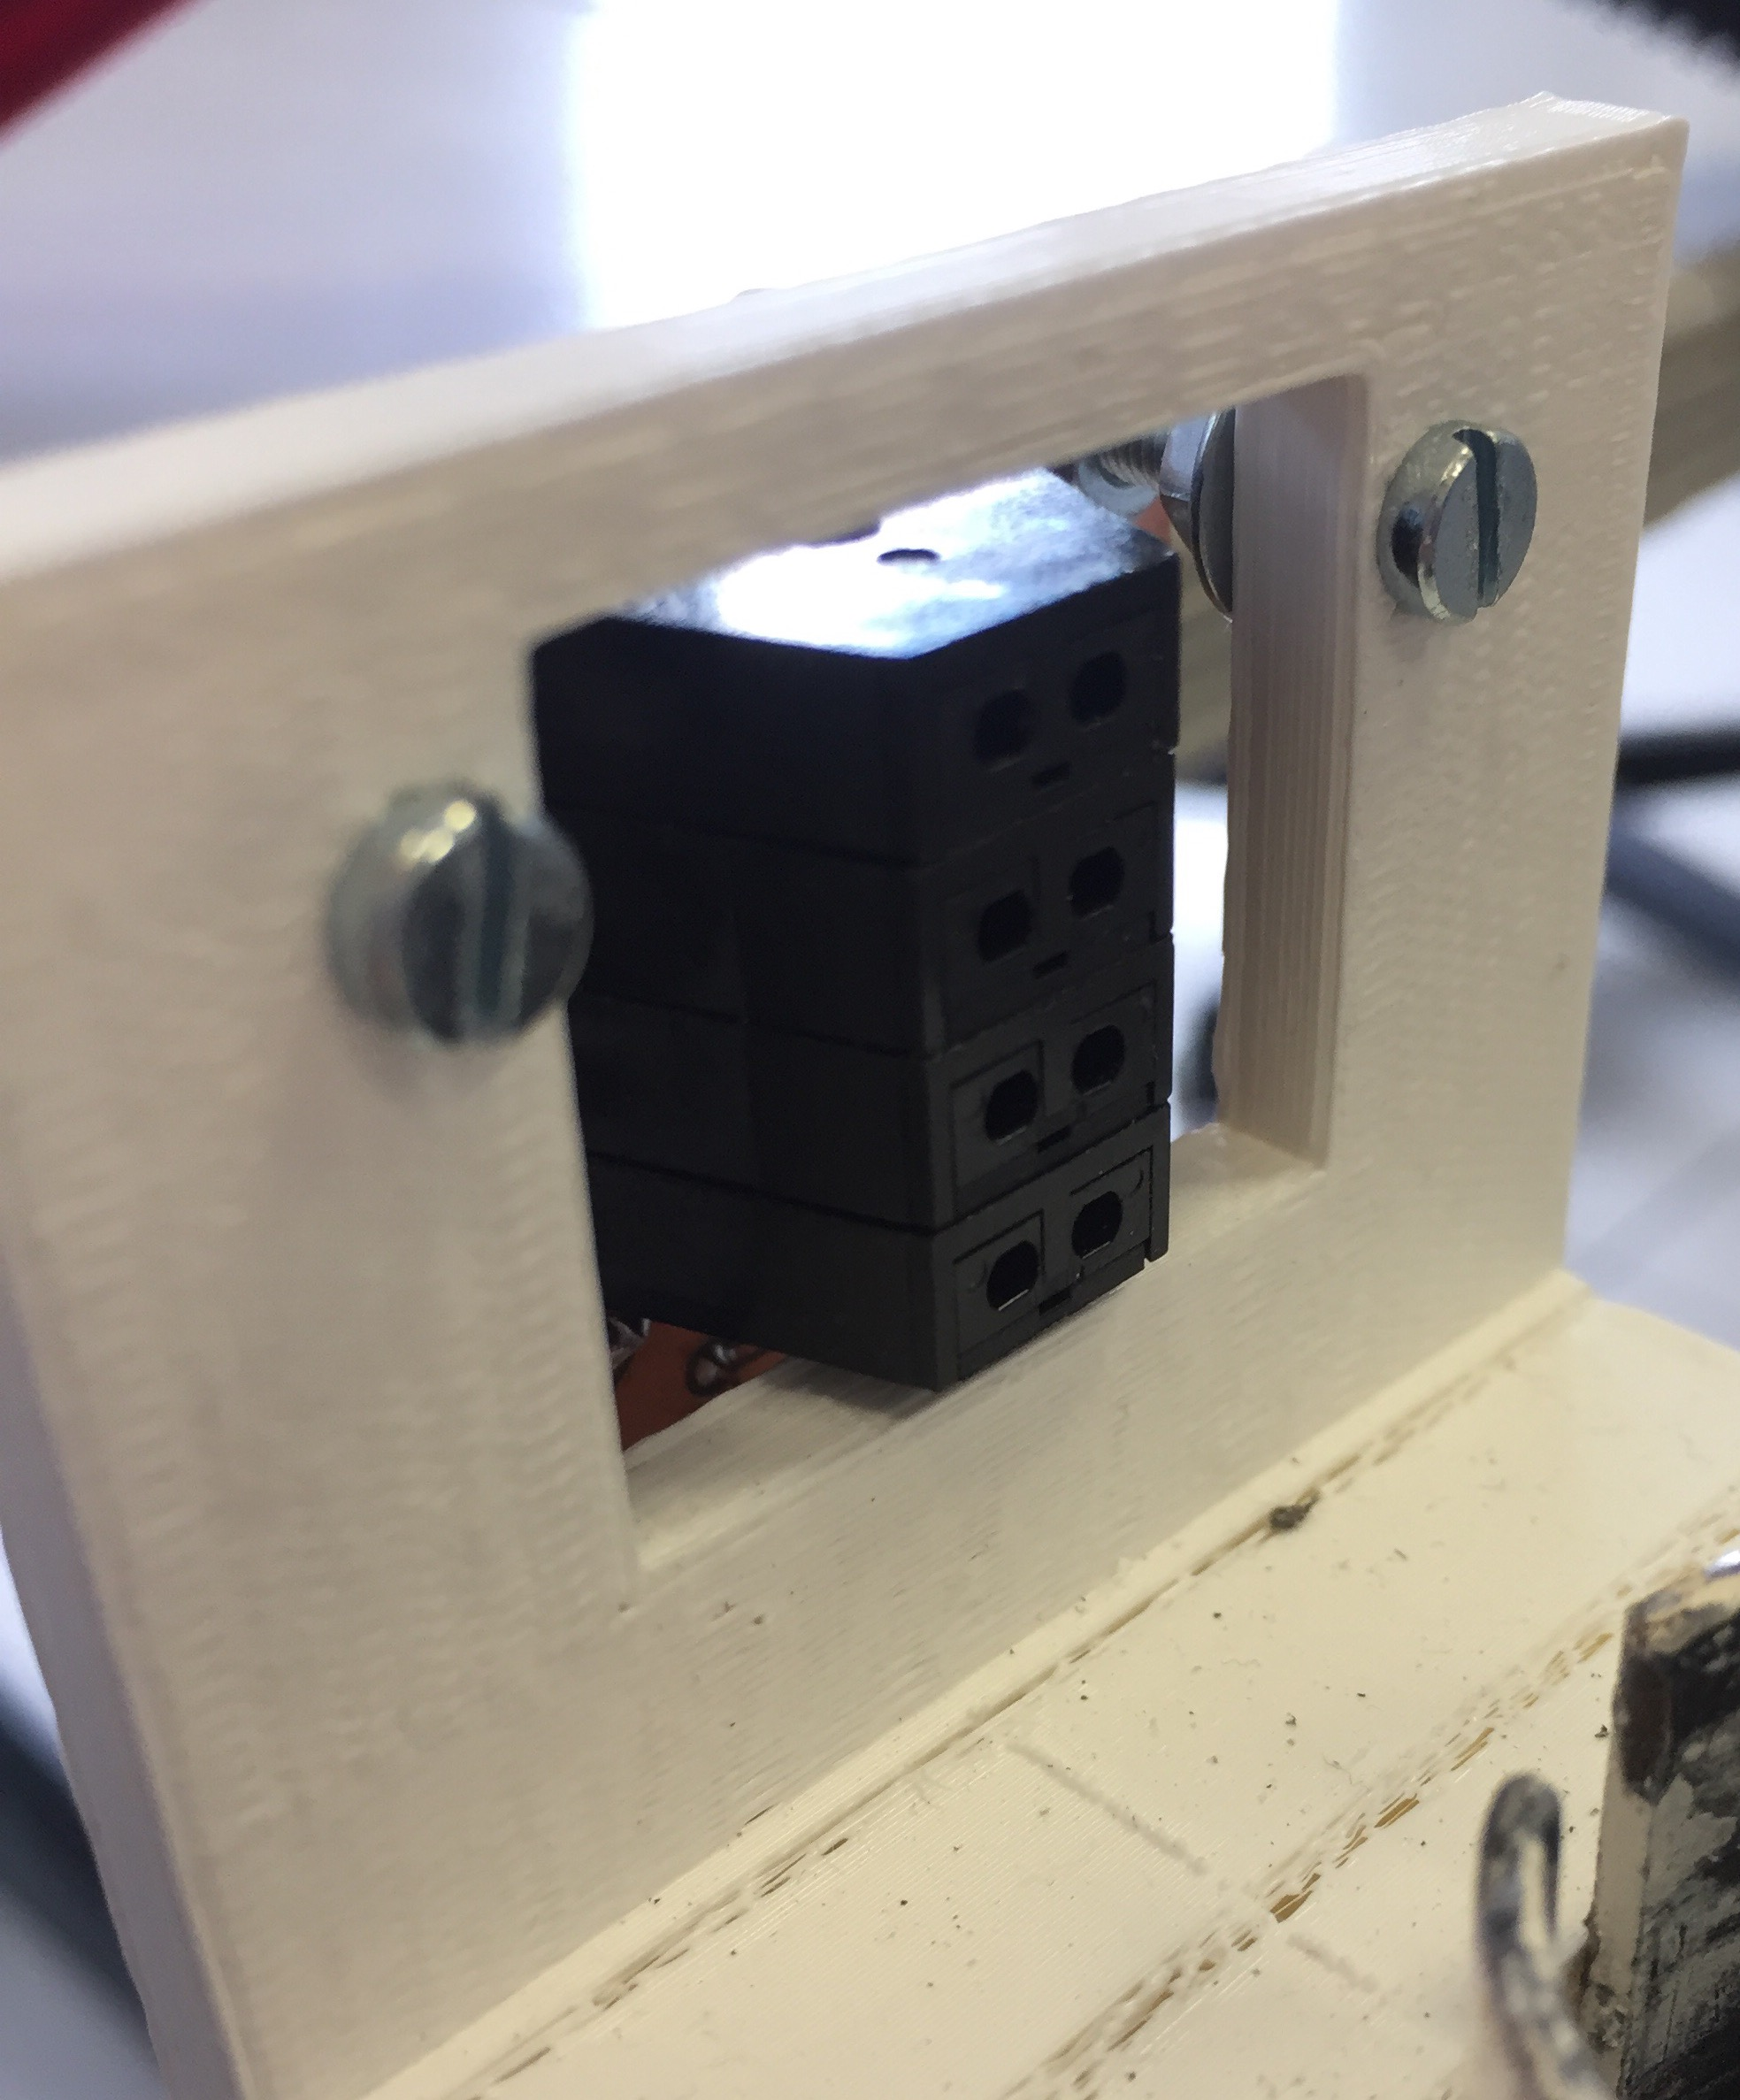
\includegraphics[height=5.5cm]{4Fotodiodi} }}%
    \subfloat[Le 16 posizioni in permutazione ciclica]{{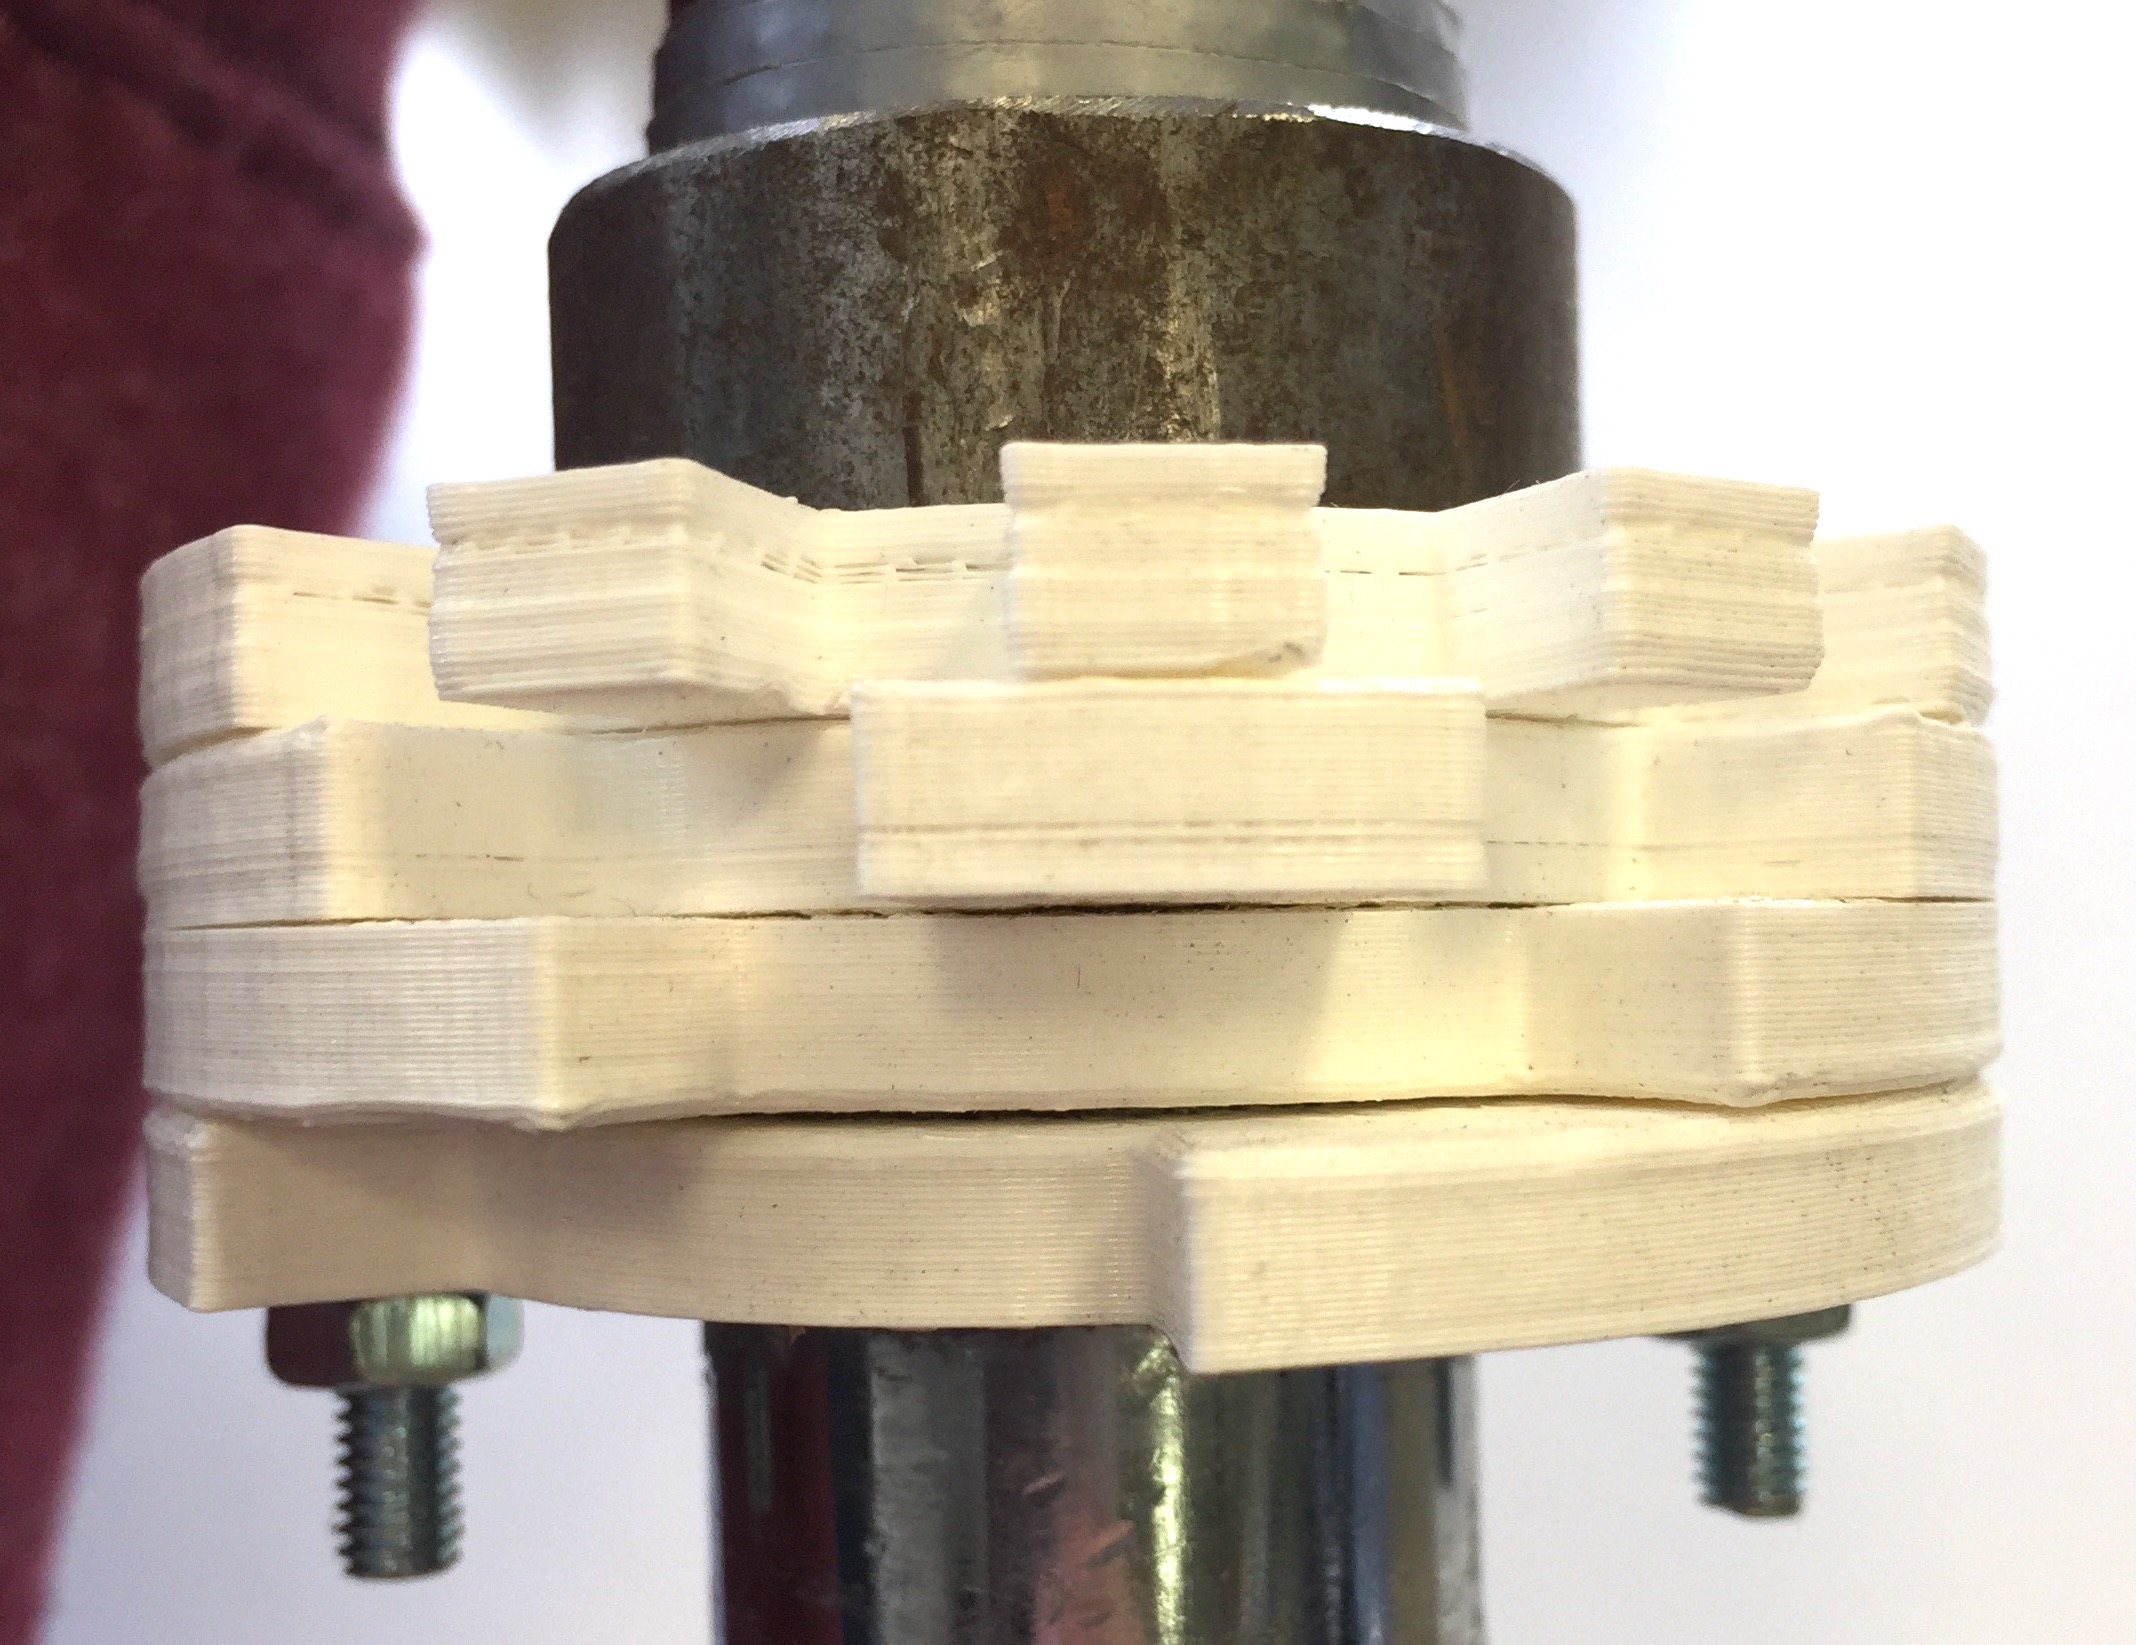
\includegraphics[height=5.5cm]{codifica4bitManubrio} }}%
    \caption{Sensori del manubrio}%
    \label{manubrio}
\end{figure}
Per ottenere le informazioni relative alla posizione del manubrio è stato scelto un angolo massimo di rotazione di 120\degree. Questo angolo è stato diviso in 16 posizioni. \\
\begin{wrapfigure}{r}{0.2\textwidth} %this figure will be at the right
    \centering
    \vspace{-1.5cm}
    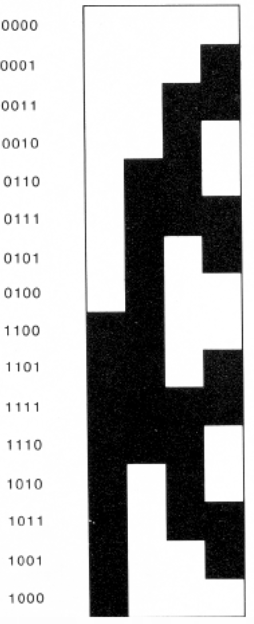
\includegraphics[width=0.2\textwidth]{codifica4bit}
\end{wrapfigure}
Per poter rilevare la posizione corrente è stata necessaria una codifica in 4 bit. Per ottenere questa codifica, si è fatto uso di 4 fotodiodi\footnote{Il fotodiodo è un particolare tipo di diodo fotorilevatore che funziona come sensore ottico sfruttando l'effetto fotovoltaico, in grado cioè di riconoscere una determinata lunghezza d'onda dell'onda elettromagnetica incidente e di trasformare questo evento in un segnale elettrico di corrente applicando ai suoi estremi un opportuno potenziale elettrico. Esso è dunque un trasduttore da un segnale ottico ad un segnale elettrico.} che permettono di rilevare i 4 spazi che compongono una delle 16 configurazioni. I fotodiodi permettono di distinguere uno spazio vuoto da uno spazio pieno creando un segnale elettrico. Le configurazioni sono state realizzate con un oggetto stampato con stampante 3D, come si vede in figura \ref{manubrio}b, in permutazione ciclica (figura a lato), che permette di accorpare gli \textit{uni} e gli \textit{zeri} e ridurre l'alternanza di \textit{vuoti} e \textit{pieni}.


\section{Sensori del volano}
\begin{figure}%

    \centering
    \subfloat[Fotodiodi]{{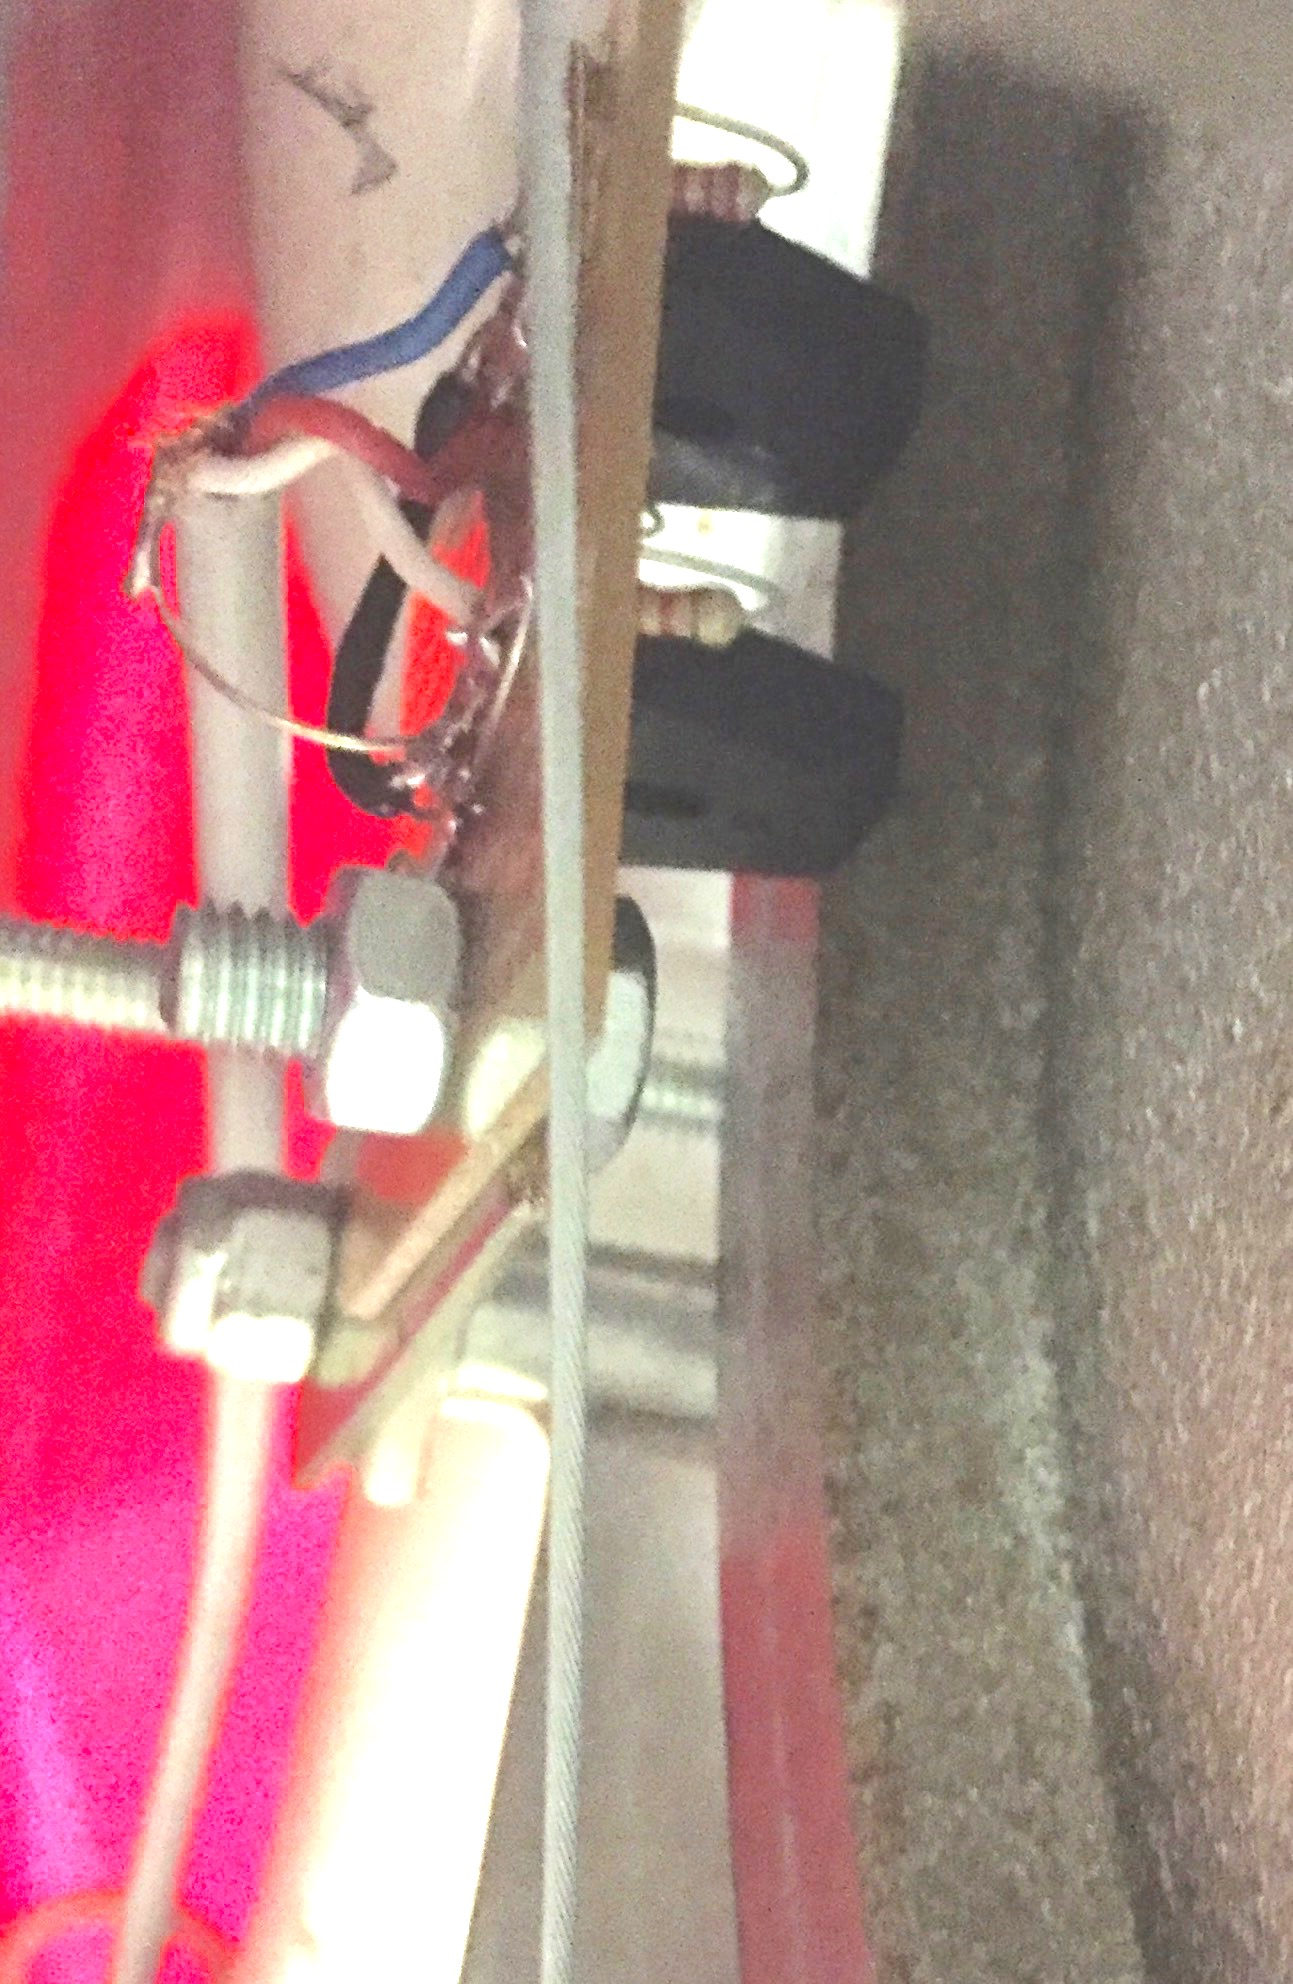
\includegraphics[height=6cm]{fotodiodivolano} }}%
    \subfloat[Polistirolo]{{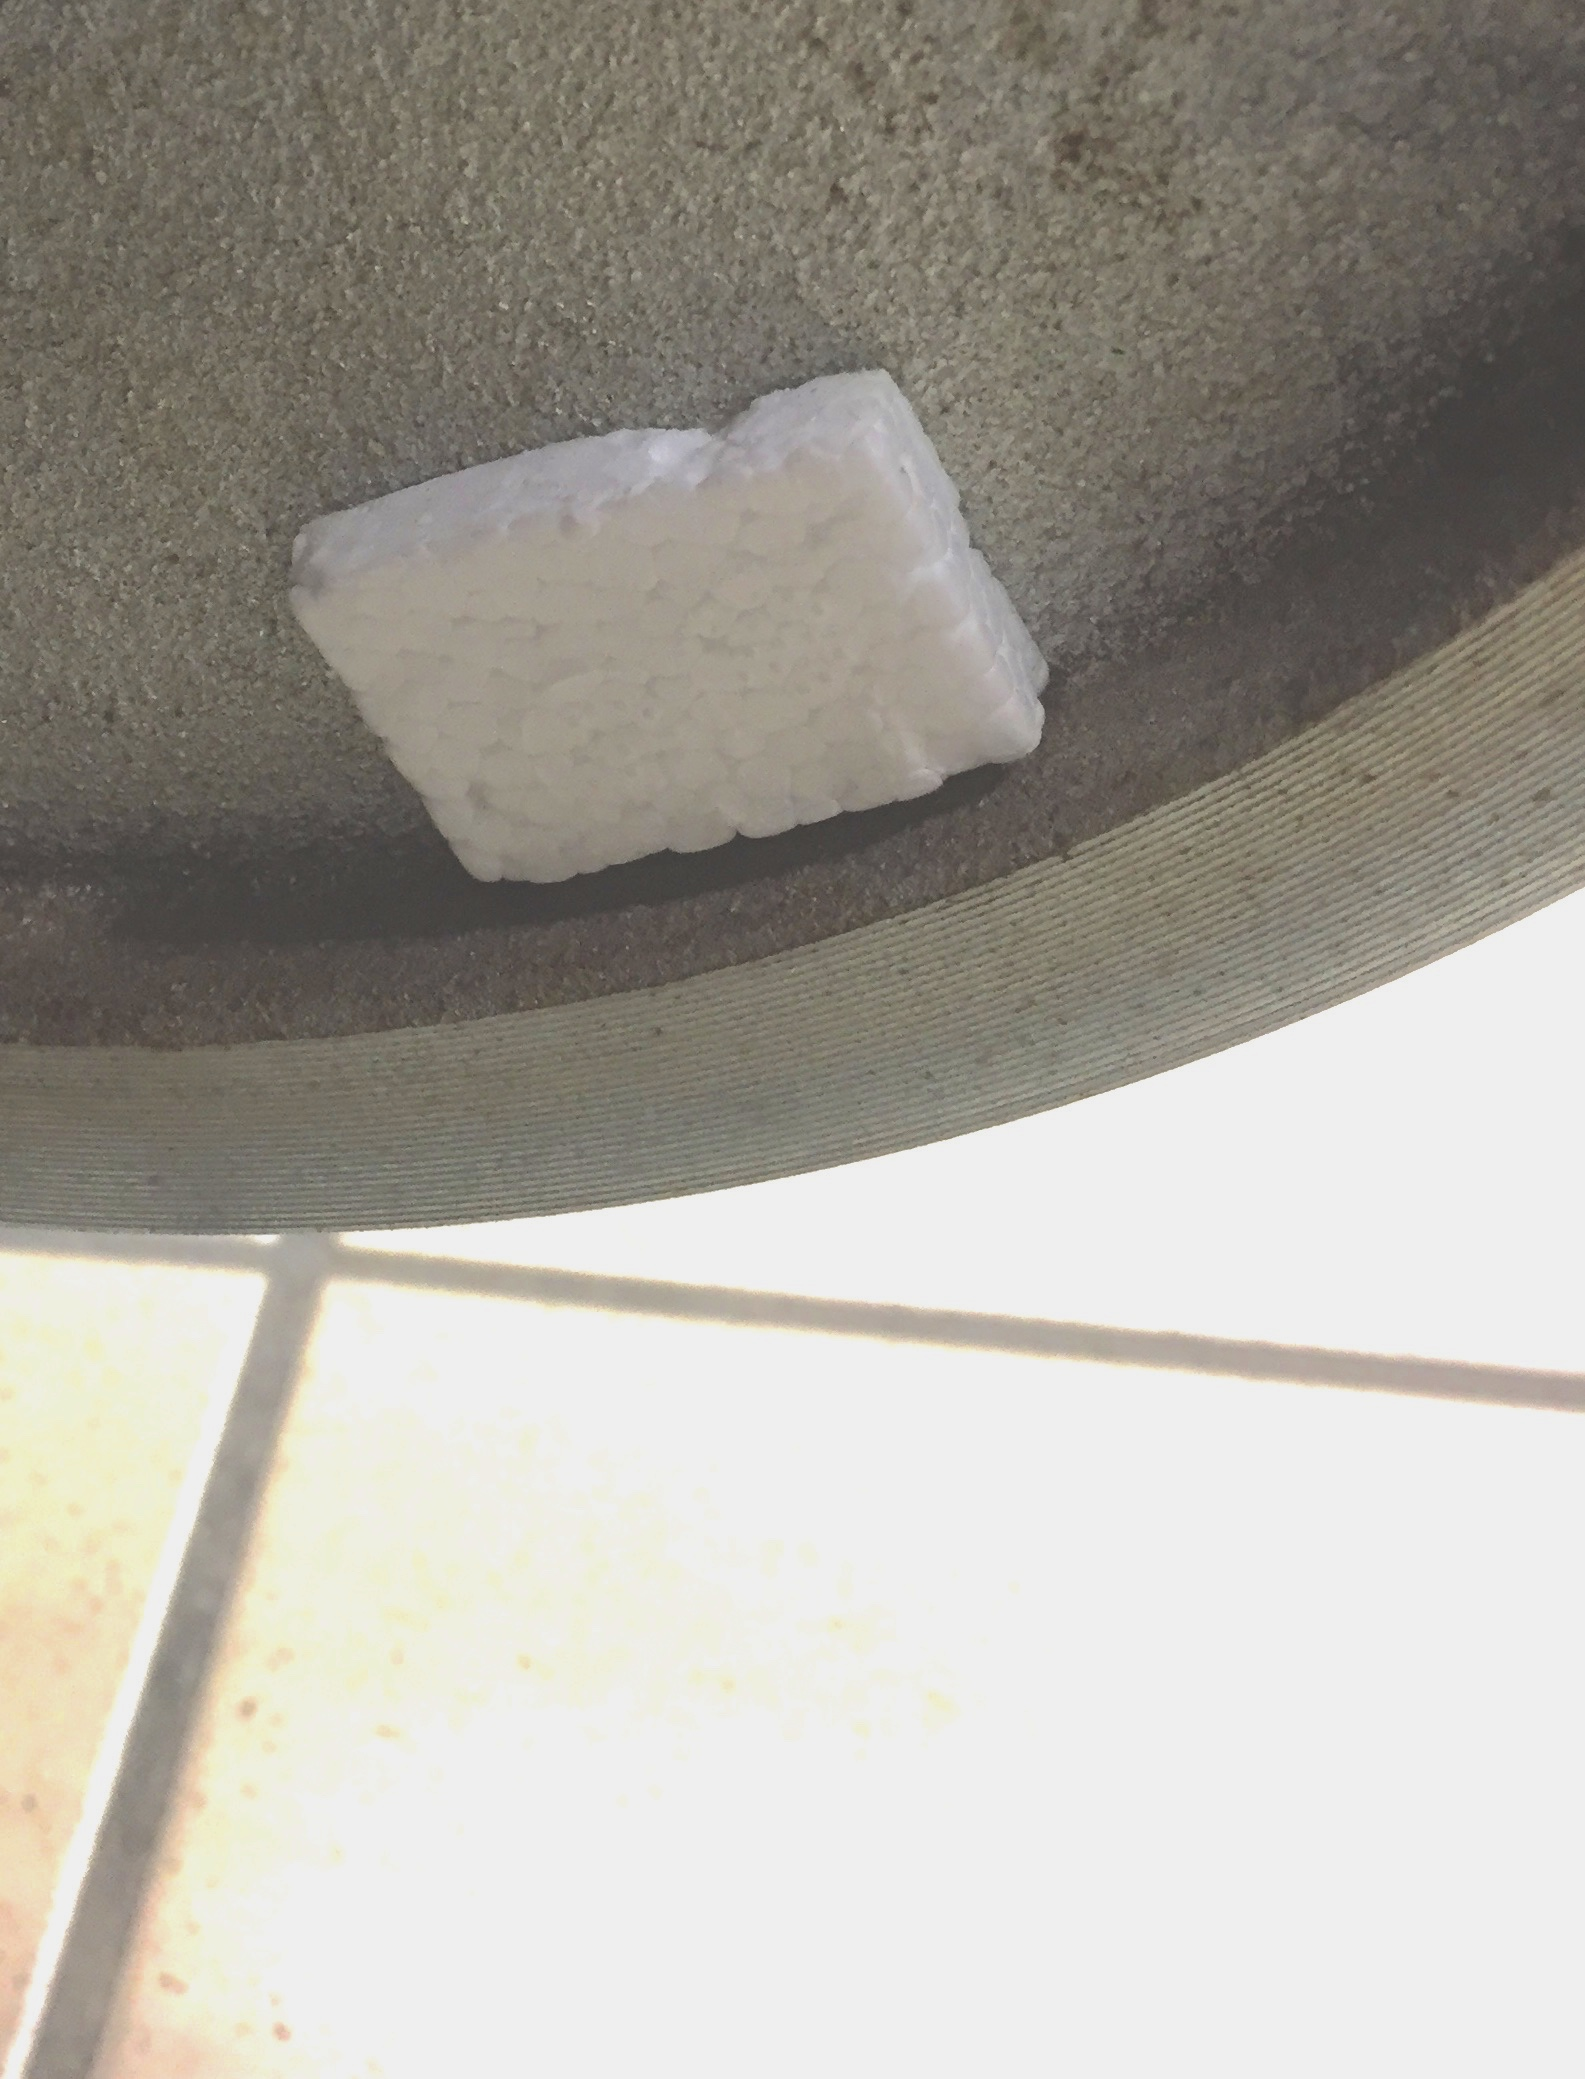
\includegraphics[height=6cm]{polistirolo} }}%
    \subfloat[Volano]{{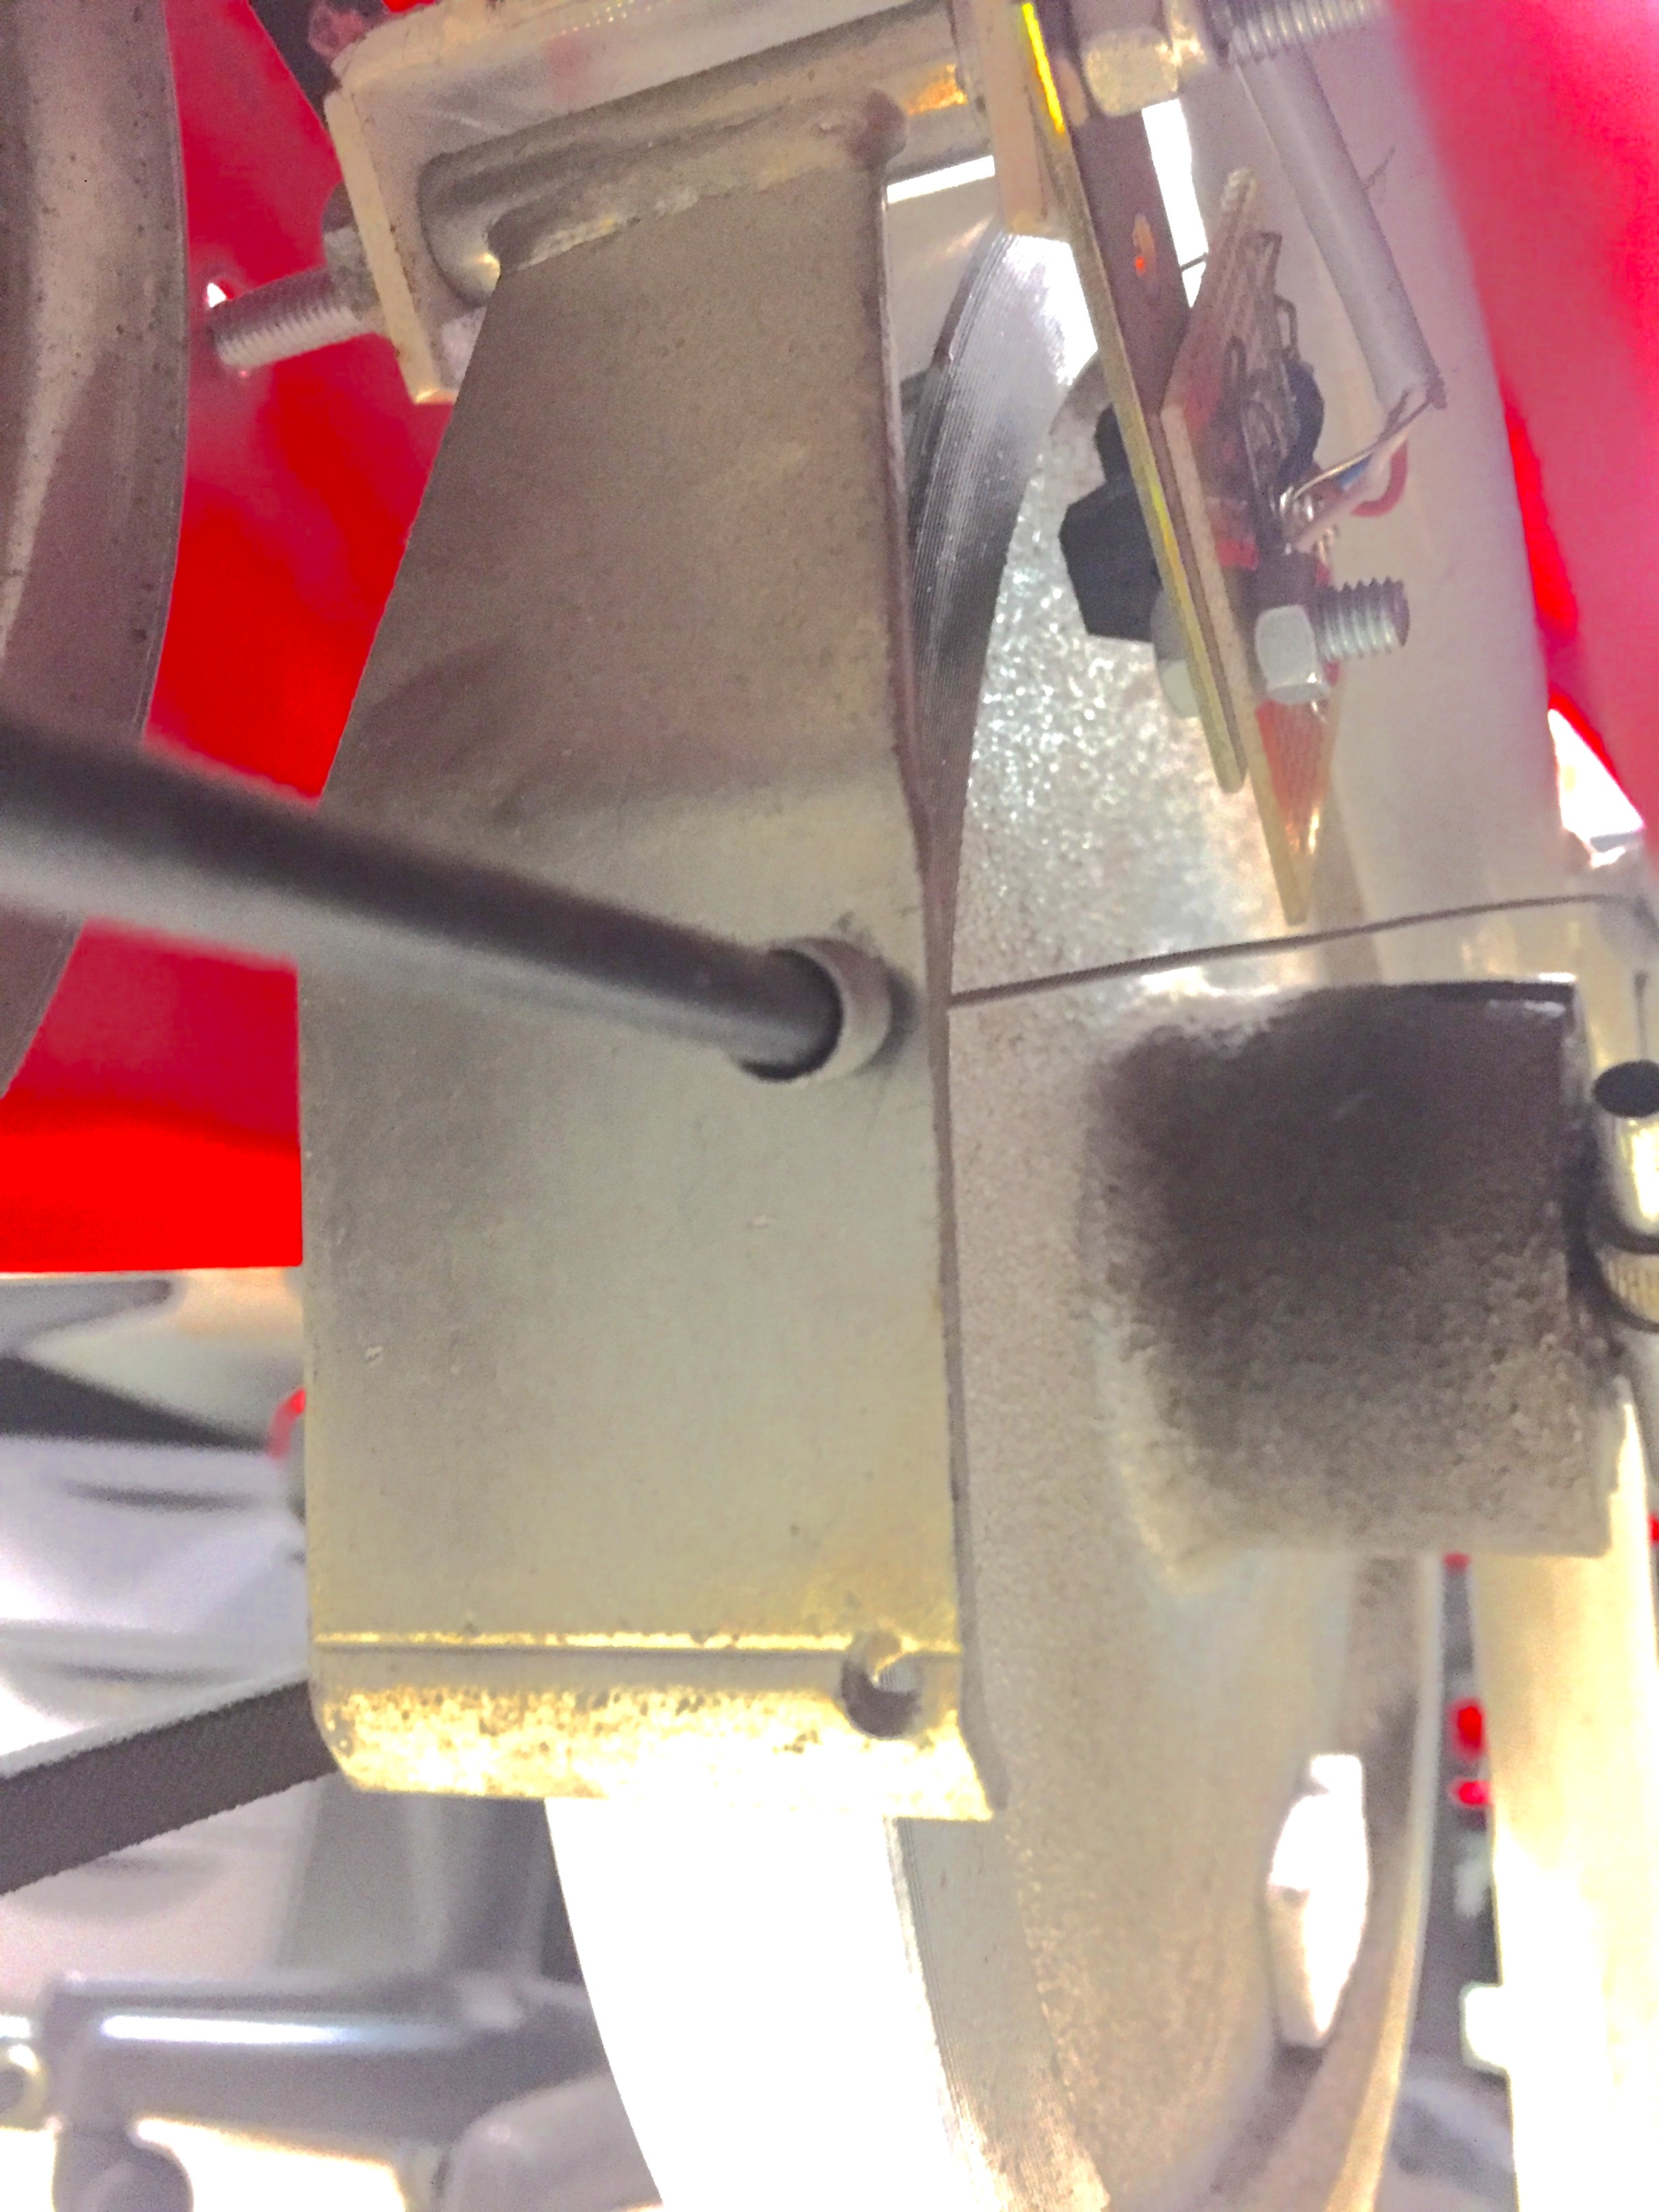
\includegraphics[height=6cm]{volano} }}%
    \caption{Sensori del volano}%
    \label{volano}
\end{figure}
La bicicletta virtuale deve muoversi ad una velocità consona alla rotazione del volano della cyclette. Quest'ultimo è stato quindi munito di un sistema che fornisce informazioni sulla velocità di rotazione. Il sistema di sensori è composto da due fotodiodi (figura \ref{volano}a) che permettono di ottenere la velocità di rotazione e distinguere se questa è oraria o antioraria. A questo fine, è stato installato sul volano un pezzo di polistirolo(figura \ref{volano}b) che permette di attivare i fotodiodi al passaggio. Grazie a questo, il microcontrollore può ottenere il tempo impiegato dal volano per coprire lo spazio che intercorre tra un fotodiodo e l'altro. La velocità di rotazione è quindi ottenuta tramite formula fisica della velocità, ovvero spazio percorso fratto tempo impiegato. La direzione di rotazione viene ottenuta distinguendo quale dei due fotodiodi viene attivato per primo. Ad esempio, se consideriamo due fotodiodi disposti orizzontalmente:\\
\begin{itemize}
  \item Se un oggetto passa da sinistra a destra, si oscurerà prima il fotodiodo sinistro poi il destro, quindi assumendo un oggetto che abbia il fulcro di rotazione sotto i fotodiodi, la sua rotazione è \textbf{oraria}
  \item in caso contrario, la rotazione è \textbf{antioraria}.
\end{itemize}
In figura \ref{volano}c si può osservare l'intero sistema del volano.

%\begin{wrapfigure}{r}{0.4\textwidth} %this figure will be at the right
%    \centering
%    \vspace{-1.3cm}
%    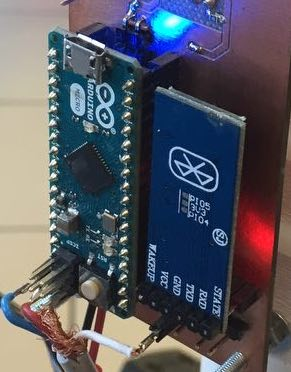
\includegraphics[height=5.5cm]{arduino}
%    \caption{La scheda Arduino Micro e il modulo bluetooth}
%    \vspace{-1.3cm}
%\end{wrapfigure}

\section{Microcontrollore}
%=========CHIEDI a lanzoni come viene ottenuto il dato dall'accelerometro e come viene ottenuto il + e il -
\noindent Il cuore della parte hardware è la scheda Arduino che elabora tutti i dati ricevuti via cavo dai fotodiodi del manubrio e del volano. Questo microcontrollore è in continua comunicazione in output con il modulo bluetooth poiché deve elaborare le informazioni che riceve dai fotodiodi ed inviarle al computer principale sotto forma di stringa.\\
 \begin{figure}[htb]
    \centering
    %\vspace{-0.7cm}
    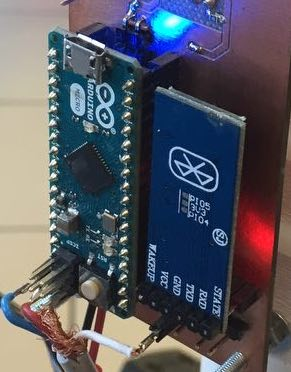
\includegraphics[height=8cm]{arduino}
    \caption{La scheda Arduino Micro e il modulo bluetooth\label{fig:arduino}}
    %\vspace{-0.3cm}
\end{figure}

\subsection{Stringa composta dal microcontrollore}
\label{stringa}
La stringa elaborata dall'Arduino è composta come segue:
\begin{itemize}
  \item \textbf{Posizione del manubrio}: un valore compreso tra 0 e 15 che indica la posizione del manubrio
  \item \textbf{Velocità di rotazione}: un valore compreso tra 0 e 40 che indica la velocità di rotazione della pedalata.
  \item \textbf{Senso di rotazione}: un segno \textbf{+} o \textbf{-} che indica senso orario o antiorario di rotazione della pedalata.
\end{itemize}

\noindent Un esempio pratico è \textbf{12+27.5}: significa che si sta registrando una pedalata in senso orario con velocità 27.5 e il manubrio è nella posizione 12.

\section{Ricevitore Bluetooth}
La ricezione della stringa avviene tramite un ricevitore bluetooth collegato ad una porta USB del computer generale in cui viene eseguito il software. Utilizzando un programma terminale apposito, chiamato HyperTerminal è stato possibile leggere la porta seriale COM a cui vengono inviati i dati a 9600 bit/s e testare la parte hardware.

\section{OSVR}
\begin{figure}[htb]
    \centering
    \vspace{-0.7cm}
    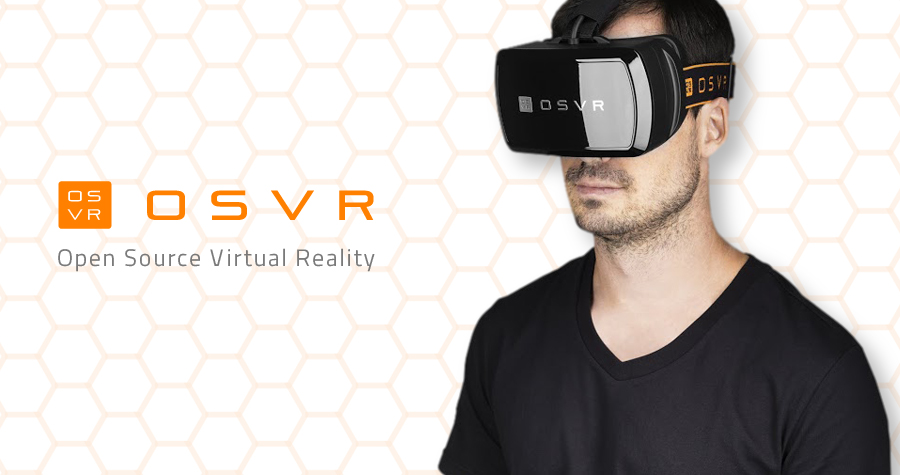
\includegraphics[width=\textwidth]{osvr1}
    \vspace{-1cm}
\end{figure}
\noindent OSVR é l'acronimo di \textit{Open-Source Virtual Reality} ed identifica la piattaforma software open-source per la Realtà Virtuale e quella aumentata. \\È stata sviluppata dalla Razer e da Sensics. La prima è l'azienda leader nel settore del gaming, mentre la seconda lo è nel settore della realtà virtuale. Affinché questa piattaforma sfondasse nel mercato, le società sopracitate hanno deciso di rendere open-source sia il software sia l'hardware per i programmatori. È infatti reperibile su github il codice sorgente. OSVR consente in modo davvero semplice la configurazione e la gestione dei vari dispositivi: occhiali VR, inseguitori di posizione, periferiche di gioco e vari altri. 

\subsection{Caratteristiche}
L'OSVR è composto da un display montato su una visiera, o meglio head-mounted (HMD), da 2 lenti amovibili, da un display OLED da 5.5 pollici con risoluzione 1920 x 1080 pixel, 60 fps di refresh rate e campo visivo di 100 gradi. Contiene una scheda madre riprogrammabile con accelerometro e giroscopio integrati. Il visore OSVR dispone di doppie lenti che consentono di ridurre la distorsione delle immagini. A differenza di altri visori, questo dispone di una cintura elastica che porta i cavi fino all'altezza delle spalle dell'utilizzatore, in modo da non limitarne il movimento e quindi l'esperienza di gioco.\\

 \begin{figure}[htb]
    \centering
    %\vspace{-0.7cm}
    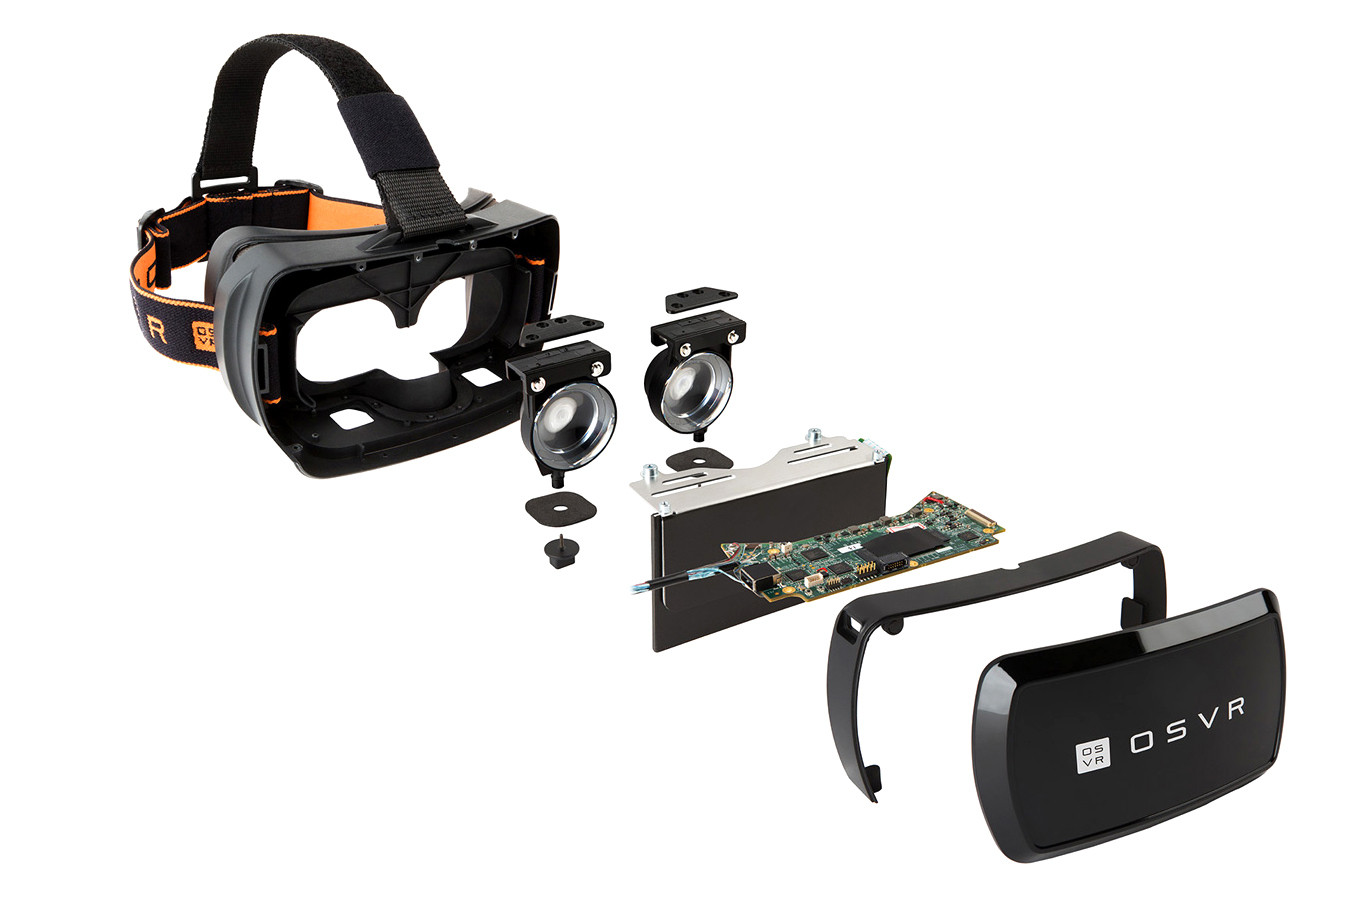
\includegraphics[height=8cm]{osvr2}
    \caption{I componenti del visore OSVR HDK1\label{fig:osvr2}}
    %\vspace{-0.3cm}
\end{figure}
\noindent Il punto forza di questa piattaforma è la facile integrazione con dispositivi e con software aggiuntivi. Ad esempio, utilizzando una telecamera eye-tracking è possibile adoperare il software fornito dal produttore della fotocamera per calcolare la direzione dello sguardo. È inoltre possibile utilizzare il visore in praticamente il 90\% dei sistemi operativi.
In questo modo lo sviluppatore non ha più bisogno di scegliere anticipatamente un particolare sistema operativo per la sua applicazione, la cui realizzazione richiederà meno tempo sfruttando i plug-in dei quali l'OSVR dispone. Si permette così allo sviluppatore di concentrarsi su essa piuttosto che sull'interfacciamento.
 Sono inoltre reperibili all'interno di Github\footnote{GitHub è un servizio di hosting per progetti software. Il nome deriva dal fatto che è un servizio sostitutivo del software dell'omonimo strumento di controllo versione distribuito, Git.}, tutti i plug-in di integrazione con i vari motori grafici quali Unity e Unreal Engine.
\subsection{Integrazione}
L'integrazione dell'OSVR verrà trattata nella sezione \textit{\nameref{software}} in cui si descriverà il procedimento per installare, configurare ed utilizzare il visore.